\documentclass [12pt] {article}

\usepackage[utf8]{inputenc}
\usepackage{graphicx}	
\usepackage[section]{placeins}

\title {LOGIC DESIGN - WEEK 3 - REPORT}
\author{Pham Duc Anh Khoa - 2053140 \\
				Nguyen Thi Ngoc Nhi - 2052632\\
				Ngo Chan Phong - 2053321 \\
				Le Hoang Minh - 2052595 \\
				Tran Hoang Minh Quan - 2053380 \\
				Phan Tien Vinh - 2052323\\
				Nguyen Tien Trung - 2052353}
\date{11 - 05 - 2021}

\begin {document}
	\pagenumbering {gobble}
	\maketitle 
	\newpage
	\pagenumbering {arabic}
	
	\section * {Work division}
		Pham Duc Anh Khoa - Doing Question 3 \\
		Nguyen Thi Ngoc Nhi - Doing Question 1 \\
		Ngo Chan Phong - Doing Question 1 \\
		Le Hoang Minh - Question 2 \\
		Phan Tien Vinh - Question 4 \\
		Nguyen Tien Trung - Doing report
		
	\section  {Answering the questions}
		\subsection {The above declaration describes flip flop with synchronous or asynchronous reset ? Explain ?}
			The above declaration describe \textbf{synchronous} reset. \\
			Explain: the \textbf{reset} condition only activate when the \textbf{clock} is positive edge (\textbf{always @(posedge clk)})\\

		\subsection {What is the active level (LOW/HIGH) of reset and set signal ?}
			\begin {itemize}
				\item \textbf{Reset} : High. When we associate HIGH with TRUE/1 it is called positive logic. HIGH is TRUE or 1 because in digital hardware the higher voltage is associated with the logic 1 state
				\item \textbf{Set} : Low. When we associate LOW with FALSE/0  it is called negative logic. LOW is FALSE or 0 because the 0 logic state in hardware is represented by the lower voltage, usually close to 0 volts.
			\end {itemize}
			
		\subsection {Between set and reset signals, which is higher priority}
		The reset signal has highest priority, because this declaration describes synchronous reset. And when asserted (=1) forces the state of the flip-flop to 0 on the rising edge of the clock. 
The set signal has priority over the d input. And when asserted forces the flip-flop to 1 on the rising-edge of the clock.

		\subsection {Could we change the operator $\Leftarrow$ by \textbf{=}? Explain ?}
		We can change the operator $\Leftarrow$ by \textbf{=}. It is Recommended to use non-blocking assignment ''$\Leftarrow$'' for sequential logic and blocking assignment "\textbf{=}" for combinational logic. \\
		We use non-blocking statement "$\Leftarrow$" to avoid race – condition. Using blocking statement "\textbf{=}" can cause a race-around condition. But the declaration above doesn’t contain any race- condition so we can replace $\Leftarrow$ by \textbf{=}, which wont be cause any big difference. 
		
		\subsection {The always block in dff sync module is triggered by level (level-sensitive) or edge (edge-sensitive) ?}
		The always block in \textbf{dff\_sync} module is triggered by \textbf{edge sensitive} (\textbf{posedge clk})
		
		\subsection{Could we change the declaration of \textbf{rq} from \textbf{reg} to \textbf{wire} ? Explain ?}
		We \textbf{cannot} change the declaration from reg to wire.\\
		\textbf{Wire}: are used for connecting different elements. They need to be driven by either continuous assign statement or from a port of a module.\\
		\textbf{Reg}: are also used for connecting but they can retain their value till next value is assigned to them, which means if it is holding some value, we should declare it as “reg”.
		
		\subsection{Could we move the place of assign lines to above always block. Does q and q bar receive the appropriate
value of rq after moving ? Explain your answer ?}
			\begin {itemize}
				\item We \textbf{cannot} move the assign line above \textbf{always} block because the flip flop should only be activated when clock is positive edge.
				\item The \textbf{q} and \textbf{q bar} will not receive the appropriate value of rq after moving, because \textbf{rq's} value is assigned in the \textbf{always} block.
			\end{itemize}
			
		\subsection{Is there any different between using the operator '' ! '' and ''$\sim$'' in this case.}
			\begin {itemize}
				\item `` ! '' stands for logical negation. `` ! '' means ``reverse value''.
 				\item ``$\sim$'' stands for bit-wise negation. ``$\sim$''' means the negation of the value.
			\end{itemize}

	\section {Implement the J-K flipflop that satisfies the following requirements:}
		\begin {itemize}
			\item Set and Reset are low-level activate. 
			\item Set has higher priority than Reset.
			\item Set is asynchronous. While Reset is synchronous.
			\item The flip-flop works at negative edge of clock.
		\end {itemize}
		
		\subsection {Simulation of the design}		
		\begin{figure}[htbp]
			\centerline{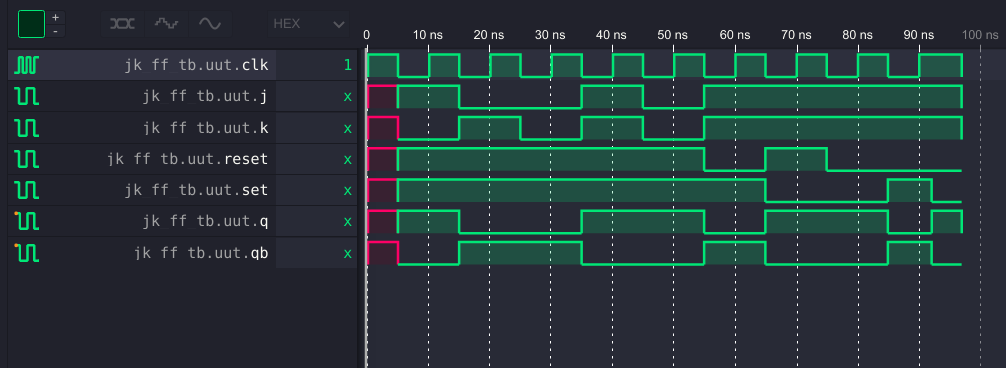
\includegraphics[scale = 0.5]{jkff.png}}
			\caption{J-K flip flop simulation.}
			\label{fig}
		\end{figure}
		
		\subsection {Simulation break down}
			\begin {itemize}
				\item From the time 0ns $\rightarrow$ 55ns: The waveform show that the design of J-K flip flop work as \textbf{negative edge}.
				\item From the time 55ns $\rightarrow$ 65ns: The waveform show that \textbf{reset} works when it is \textbf{active - low}.
				\item From the time 65ns $\rightarrow$ 75ns: The waveform show that \textbf{set} works when it is \textbf{active - low}.
				\item From the time 75ns $\rightarrow$ 85ns: The waveform show that \textbf{set} has higher priority than \textbf{reset}.
				\item From the time 85ns $\rightarrow$ 100ns: The waveform show that \textbf{set} is \textbf{asynchronous}.
			\end {itemize}
			
	\section{Design and implement 4-bit synchronous counter that satisfy the following requirement:}
		\begin {itemize}
			\item Full counter (from 0 to 15). 
			\item Using \textbf{only structural model}. (You can reuse the dff sync module our your implemented JK-flip flop).
			\item Prototype: module counter(clk, count, RCO), where: \\
				$\rightarrow$ \textbf{clk}: the input clock.\\
				$\rightarrow$ \textbf{count}: the count output.\\
				$\rightarrow$ \textbf{RCO}: is 1 when the value of the counter is 15, 0 otherwise.\\
		\end{itemize}
		
		\subsection {Simulation of the design}		
		
%			\begin{figure}[!htb]
%				\centerline{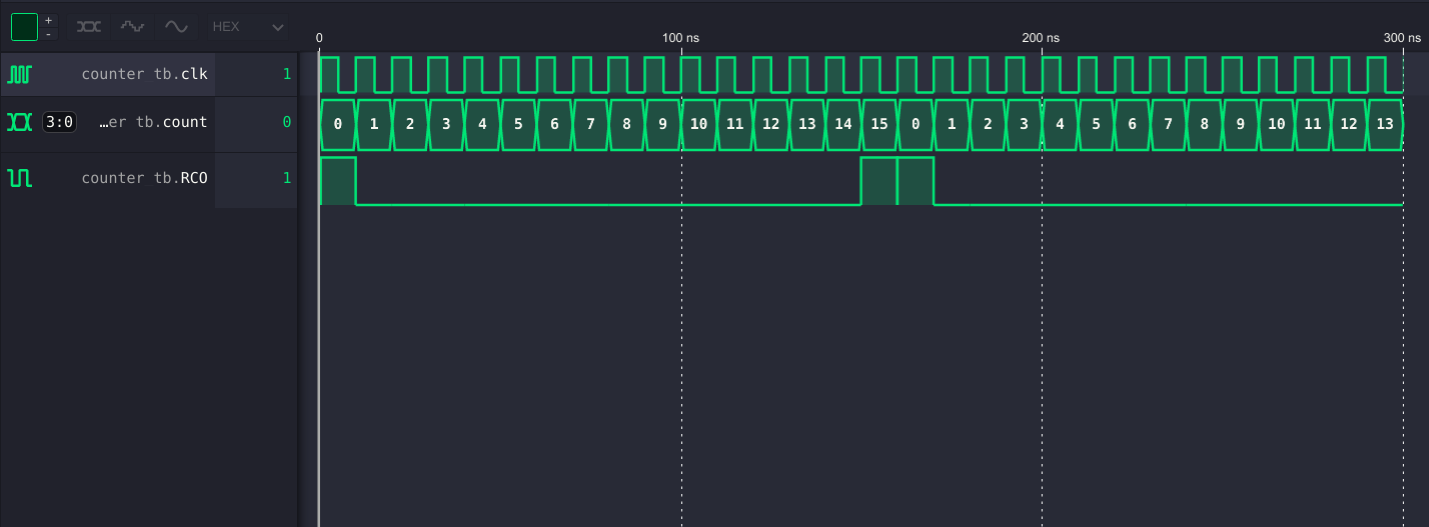
\includegraphics[scale = 0.35]{counter.png}}
%				\caption{4 bit synchronous counter.}
%				\label{fig}
%			\end{figure}
			\centerline{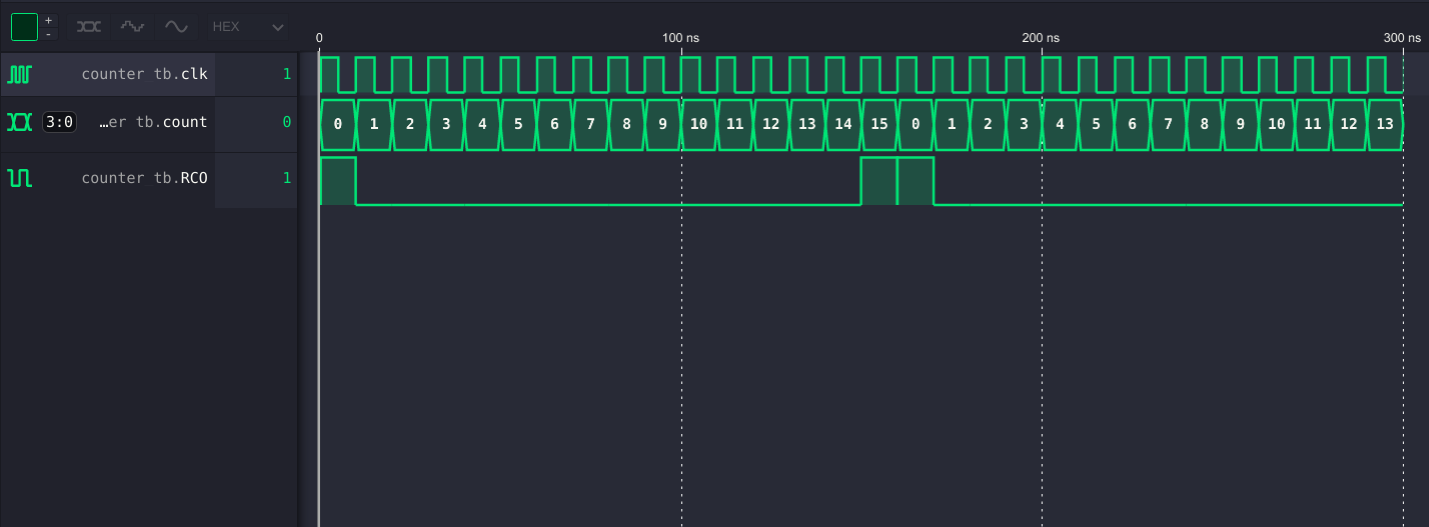
\includegraphics[scale = 0.35]{counter.png}}
			\centerline{Figure 2: 4 bit synchronous counter} 

		\subsection {Simulation break down}
			\begin {itemize}
				\item From the time 0ns $\rightarrow$ 155ns: The waveform show that the design of 4 bit synchronous counter works properly.
				\item From the time 155ns $\rightarrow$ 165ns: The waveform show that \textbf{RCO} works properly when count is 15 or 0.
			\end {itemize}
		 
		 \section{Redesign the question 3 by using either RTL or Behavioral model:}
		
		\subsection {Simulation of the design}		
		
%			\begin{figure}[!htb]
%				\centerline{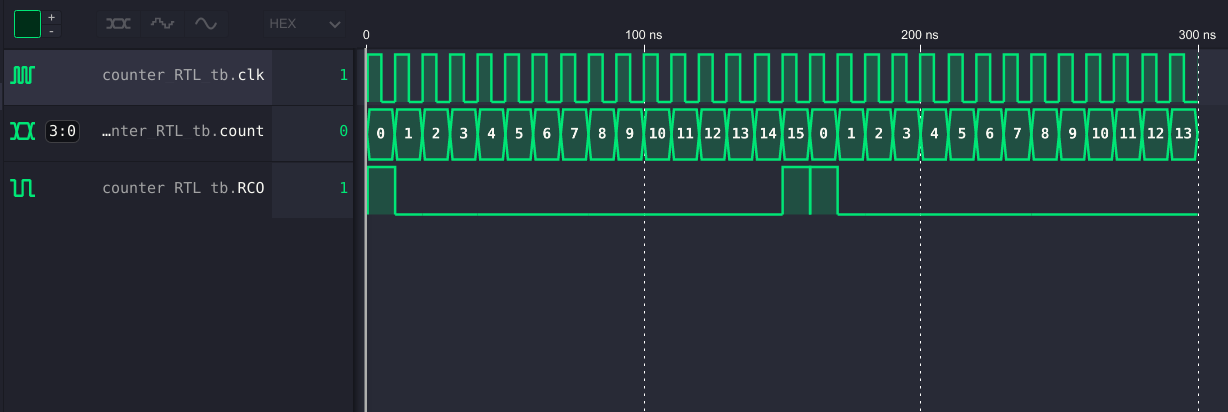
\includegraphics[scale = 0.35]{counter_RTL.png}}
%				\caption{4 bit synchronous counter with RTL structure.}
%				\label{fig}
%			\end{figure}
			\centerline{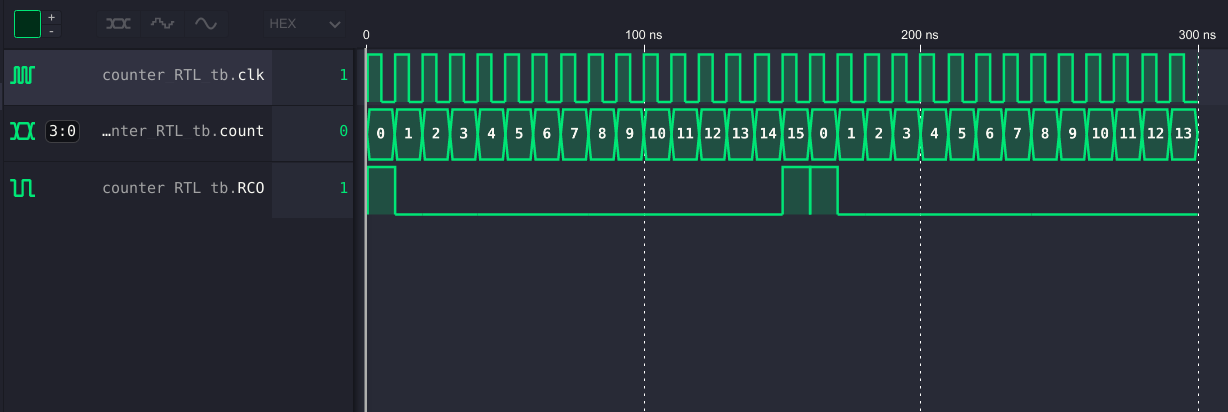
\includegraphics[scale = 0.35]{counter_RTL.png}}
			\centerline{Figure2: 4 bit synchronous counter with RTL structure.} 

		\subsection {Simulation break down}
			\begin {itemize}
				\item The waveform show that the design works just like the design on Question 3.
			\end {itemize}
		

\end{document}